%***********************************************************************
% Lab Report Template
% R. W. Melton
% May 19, 2019
% August 24, 2020
%***********************************************************************
%Modify the following macros to set document property values
%used for cover sheet (title page) and page header
\newcommand{\CourseNumber}{CMPE-250}
\newcommand{\CourseName}{Assembly and Embedded Programming}
\newcommand{\SemesterName}{Fall 2020}
\newcommand{\SemesterCode}{20201}
\newcommand{\LabExNum}{5}
\newcommand{\LabExTitle}{Secure String I/O and Number Output}
\newcommand{\StudentName}{Andrei Tumbar}
\newcommand{\DateSubmit}{Submitted: 09-29-20}
\newcommand{\LabSection}{5}
\newcommand{\LabInstructor}{Gordon Werner}
\newcommand{\TAa}{Tianran Cui}
\newcommand{\TAb}{Anthony Bacchetta}
\newcommand{\LectureSection}{1}
\newcommand{\LectureInstructor}{Melton}
%End macros for document property values
%***********************************************************************
\title{Lab Ex. \LabExNum\ Report}
\author{\StudentName}
\date{\DateSubmit}
\makeatletter %make \title, \author, and \date availabile with \@
\newcommand{\FontSize}{12}
\newcommand{\FontUnit}{pt}
\newcommand{\HeadSize}{\dimexpr \FontSize\FontUnit + 2pt \relax}
\documentclass[\FontSize\FontUnit,letterpaper,oneside]{article}
\usepackage[twoside=false,margin=1in]{geometry}
\usepackage[utf8]{inputenc}
\usepackage[USenglish]{babel}
\usepackage{graphicx}
\usepackage[normalem]{ulem}
\usepackage{newtxtext, newtxmath}
%If newtx package had to be installed in multiuser environment
%regular user may have to run updmap command to avoid following error
%FATAL:  ``PK font ts1-qtmr could not be created.'' in miktex-makepk
%Alternatively, uncomment the following line
%\pdfmapfile{=pdftex35.map
\usepackage{booktabs}
\usepackage{enumitem}
\usepackage{nameref}
\usepackage[pdfborder={0 0 0},plainpages=false,pdfpagelabels]{hyperref}
\def\code#1{\texttt{#1}}
%If hyperref generates errors on first build, rebuild.            
\hypersetup{pdfauthor={\@author},
            pdftitle={\@title},
            pdfsubject={\CourseNumber\ \SemesterCode},
            %pdfkeywords={},
            %pdfproducer={Latex with hyperref, or other system},
            %pdfcreator={pdflatex, or other tool}
            urlcolor=none}
\setlength{\topsep}{\z@}
\setlength{\partopsep}{\z@}
\setlength{\itemsep}{\z@}
\setlength{\parindent}{\z@}
\setlength{\parskip}{\FontSize\FontUnit plus 2pt minus 1pt}
\setlength{\baselineskip}{\dimexpr \FontSize\FontUnit + 2pt \relax}
\renewcommand \baselinestretch{1}
\makeatletter
  \renewcommand \section{
    \@startsection{section}{1}{\z@}
      %Before 2 lines, accounting for normal \parskip
      {\dimexpr \FontSize\FontUnit * 2 - \parskip \relax plus 0pt minus 0pt}
      %After 1 line, accounting for normal \parskip
      {0.1pt plus 2pt minus 1pt} %nonzero amount to get normal \parskip
      {\normalfont\normalsize\bfseries}} 
  \renewcommand \subsection{
    \@startsection{paragraph}{2}{\z@}
      %Before 1 lines, accounting for normal \parskip
      {0.1pt plus 2pt minus 1pt}
      %After 0.5 em on same line as heading
      {-0.5em} 
      {\normalfont\normalsize\bfseries}} 
  \renewcommand \subsubsection{
    \@startsection{paragraph}{3}{\z@}
      %Before 1 line, accounting for normal \parskip
      {0.1pt plus 2pt minus 1pt}
      %After 0.5 em on same line as heading
      {-0.5em} 
      {\normalfont\normalsize\uline}} 
  \renewcommand \paragraph{
      \@startsection{paragraph}{4}{\z@}
      %Before 1 line, accounting for normal \parskip
      {0.1pt plus 2pt minus 1pt}
      %After 0.5 em on same line as heading
      {-0.5em} 
      {\normalfont\normalsize}} 
\makeatother
\pagenumbering{arabic}
\headheight=\HeadSize
\usepackage{fancyhdr}
\renewcommand{\headrulewidth}{0pt}
\renewcommand{\footrulewidth}{0pt}
\makeatletter %make \title, \author, and \date availabile with \@
\pagestyle{fancy}
\fancyhead{} %clear all header fields
\fancyhead[L]{\small \CourseNumber\ \SemesterCode \@author:  \@title}
\fancyhead[R]{\small Page \thepage\ of \pageref*{LastPage}}
\fancyfoot{} %clear all footer fields
\fancypagestyle{plain}{
  \renewcommand{\headrulewidth}{0pt}
  \renewcommand{\footrulewidth}{0pt}
  \fancyhf{} %clear header and footer fields
  \fancyfoot[C]{\small \CourseNumber\ \SemesterCode\ \@author:  \@title:  
    Page \thepage\ of \pageref*{LastPage}}
}
%May require second build to get correct page numbers.   


\usepackage{xcolor}
\usepackage{listings}

\definecolor{mGreen}{rgb}{0,0.6,0}
\definecolor{mGray}{rgb}{0.5,0.5,0.5}
\definecolor{mPurple}{rgb}{0.58,0,0.82}
\definecolor{backgroundColour}{rgb}{0.95,0.95,0.92}

\lstdefinestyle{CStyle}{
    commentstyle=\color{mGreen},
    keywordstyle=\color{magenta},
    numberstyle=\tiny\color{mGray},
    stringstyle=\color{mPurple},
    basicstyle=\footnotesize,
    breakatwhitespace=false,         
    breaklines=true,                 
    captionpos=b,                    
    keepspaces=true,                 
    numbers=left,                    
    numbersep=5pt,                  
    showspaces=false,                
    showstringspaces=false,
    showtabs=false,                  
    tabsize=2,
    language=C
}

         
\begin{document}
\raggedbottom
\widowpenalties 1 10000
\lefthyphenmin=4
\righthyphenmin=4
\setlist{nolistsep}
%***********************************************************************
%Title page is automatically generated from macros at top of file
\pagenumbering{roman}
\begin{titlepage}
  %No space before paragraph at top of page
  %\vspace{\dimexpr-2\parsep-2\parskip\relax}
  %1.5 in before center (list) at top of page
  \vspace*{\dimexpr 1.5in - \topsep - \partopsep - \topskip - \parskip \relax}
  \begin{center}
    \textbf{\large\CourseNumber\ \CourseName\linebreak
      \linebreak
      Laboratory Exercise \LabExNum\linebreak
      \linebreak
      \LabExTitle}
  \end{center}
  \vspace*{\dimexpr 1.5in - \topsep - \partopsep - \topskip \relax}
  \par By submitting this report, I attest that its contents are wholly 
    my individual writing about this exercise and that they reflect 
    the submitted code.  I further acknowledge that permitted 
    collaboration for this exercise consists only of discussions of 
    concepts with course staff and fellow students.  Other than code 
    provided by the instructor for this exercise, all code was 
    developed by me.
  \null
  \vspace*{4\parskip}
  \hspace*{3.25in}\begin{tabular}[t]
    {@{\hskip0pt}r    %Specification
     @{\hskip1em}l    %Value
     @{\hskip0pt}}
    \toprule[1pt]
    \multicolumn{2}{l}{\StudentName}\\
    \multicolumn{2}{l}{\DateSubmit}\\
    \\
    Lab Section:&\LabSection\\
    Instructor:&\LabInstructor\\
    TA:&\TAa\\
    &\TAb\\
    \\
    Lecture Section:&\LectureSection\\
    Lecture Instructor:&\LectureInstructor
  \end{tabular}
\end{titlepage}
\pagenumbering{arabic}
\thispagestyle{plain}
%***********************************************************************
%Report body begins here
\section*{Results}
A screen capture of the memory contents after program execution was taken.

\begin{figure}[h!]
	\centering
	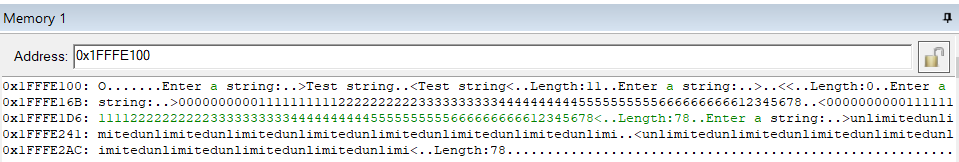
\includegraphics[width=\textwidth]{mem_cap}
	\caption{Memory after program execution}
	\label{fig:capture1}
\end{figure}

Figure \ref{fig:capture1} shows the memory contents of the program after execution. Because \code{Exercise05\_Lib.lib} attached a large portion of RAM to \code{0x1FFFE100}, the command-line output was stored in memory at the offset shown.

A capture of the register values was taken at the end of execution.

\begin{figure}[h!]
	\centering
	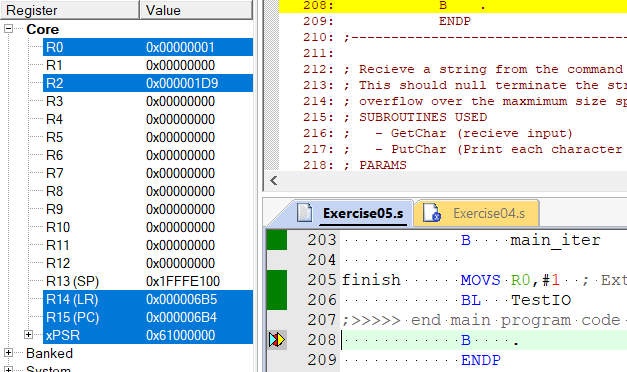
\includegraphics[]{reg_cap.png}
	\caption{Register values after program executation.}
	\label{fig:reg}
\end{figure}

Figure \ref{fig:reg} shows the register values after the code was executed. The registers to note are \code{R1} and \code{R2}. \code{R1}'s value of \code{0x0} indicate that the code is testing data using the extra-credit version of \code{PutNumU}. \code{R2}'s value of \code{0x1D9} indicates that the program has valid output given the extra-credit \code{PutNumU} subroutine was used.

\pagebreak

A screen capture of the listing as well as part of the memory map was taken.

\begin{figure}[h!]
	\centering
	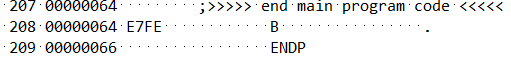
\includegraphics[]{end_offset}
	\caption{Code offset of main program end.}
	\label{fig:prog}
\end{figure}

Another screen capture was taken of the memory map after compiling the
assembly code to determine the memory regions of the generated machine-code.

\begin{figure}[h!]
	\centering
	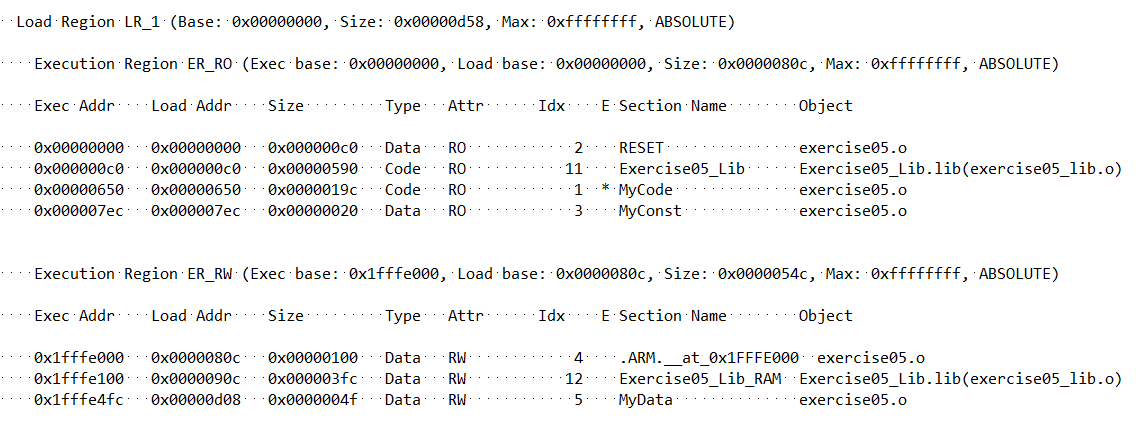
\includegraphics[width=\textwidth]{mem_map.png}
	\caption{Memory map of the assembly program.}
	\label{fig:memmap}
\end{figure}


Looking at Figure \ref{fig:prog} and Figure \ref{fig:memmap} the main program starts at address \code{0x650} and ends \code{0x66} bytes later at \code{0x6b6} because the last instruction in of the main program has an offset of \code{0x66}.


According to Figure \ref{fig:memmap} the \code{MyCode AREA} starts at \code{0x650} and ends at \code{0x7ec}. Constants starts immediately after at \code{0x7ec} and ends 32 bytes after at \code{0x80c}. 

The variables in this program don't start at the usual \code{0x1fffe100} because the \code{Exercise05\_Lib.lib} attached its own variables at this location. The memory defined by \code{Exercise05\_Lib.lib} includes a large buffer used for string output to create a virtual terminal output. Instead the variables defined in \code{Exercise05.s} start at \code{0x1ffe4fc} and end at \code{0x1ffe54b}.

A screen capture was taken to outline the code sizes of the subroutines.
\begin{figure}[h!]
	\centering
	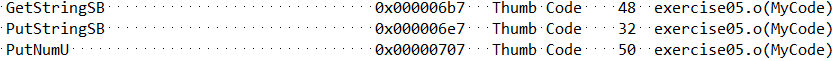
\includegraphics[width=\textwidth]{code_size.png}
	\caption{Code size of written subroutines.}
	\label{fig:sizes}
\end{figure}

Figure \ref{fig:sizes} shows the code size of \code{GetStringSB}, \code{PutStringSB} and \code{PutNumU} (with extra-credit). Sizes are listed in decimal and are $48$, $32$, and $50$ for \code{GetStringSB}, \code{PutStringSB} and \code{PutNumU} respectively.

\section*{Questions}
\begin{enumerate}
\item{Why does the number of input characters stored in the string have to be one fewer than the number of bytes allocated for the string?}

The standard for a string is to add a null terminator at the end of the string. This is so that variable length string can be stored into an array of constant size and the its length does not need to be held elsewhere. The number of characters stored must include the null terminator and therefore the number of readable characters must be 1 less than the buffer size.

\item{Why does \code{MAX\_STRING} need to be defined as an EQUate rather than as a DCD in the \code{MyConst AREA}, (i.e., a constant)?}

\code{MAX\_STRING} must be used at compile time. The \code{MyConst AREA} is stored in ReadOnly RAM and the assembler will not read RAM at compile time. The \code{EQU} instruction is a directive expanded by the assembler and can be used as a compile time constant.
\end{enumerate}


\label{LastPage}
\end{document}
